\section{Model Description}

The eclipse module is responsible for determining whether or not a spacecraft is within the shadow of a solar eclipse and if so, how much. The module finds the states of the sun, spacecraft and planets of interest, allowing each body's postition to be related and the construction of the conical shadow model. This provides the means for computing what percent of the spacecraft is illuminated where a shadow factor of 0.0 represents a total eclipse and 1.0 represents no eclipse.

To determine the states of the bodies in question, messages are passed into the code. For the spacecraft, Cartesian vectors provide the position and velocity of its center of mass. For the sun and planets, a time is chosen and input into the module along with SPK, LSK, and PCK files, indicating ephemeris data, leapsecond information, and reference frame orientation. The planets desired to be used in the module are specified through the Basilisk messaging system, where corresponding strings (e.g. "venus", "earth", or "mars barycenter") are input as Spice Objects. This allows the state data to be obtained at the given time, using Spice and the kernel files. The kernels used when testing are given in the Test Parameters section. Fig. \ref{fig:ConShad} illustrates how the states are represented and will be identified in the mathematical model. Calculations in this model are taken from Montenbruck and Gill's \textit{Satellite Orbits Models, Methods and Applications} text \cite{bib:1}.
\begin{figure}[ht]
	\centering
	\captionsetup{justification=centering}
	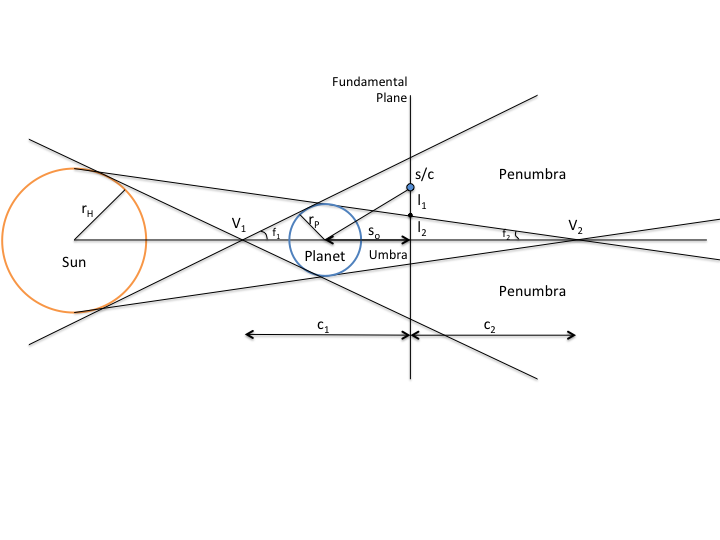
\includegraphics[width=0.9\textwidth]{Figures/conical_shadow.png}
	\caption{Representation of a Conical Shadow}\label{fig:ConShad}
\end{figure} 
\subsection{Mathematical model}

\subsubsection{Determining States}
The initial step in the eclipse module is to obtain the celestial bodies' state data and transform them into usable terms. The relationships shown below remove the dependancy on relating position to the inertial frame \textit{N} and instead utilize the planet \textit{P}, spacecraft body \textit{B}, and helio \textit{H} frames.
\begin{equation} \label{eq:1}
\bm{s}_{P/H} = \bm{r}_{N/H} - \bm{r}_{N/P}
\end{equation}
\begin{equation} \label{eq:2}
\bm{r}_{B/H} = \bm{r}_{N/H} - \bm{r}_{N/B}
\end{equation}
\begin{equation} \label{eq:3}
\bm{s}_{P/B} = \bm{r}_{N/B} - \bm{r}_{N/P}
\end{equation}

The previous three equations provide coordinates for the sun with respect to both the occulting planet and occulted spacecraft as well as the spacecraft's position with respect to the planet, respectively. The parameters on the right side of these equations come from the input state data where $\bm{r}_{N/H}$, $\bm{r}_{N/P}$, and $\bm{r}_{N/B}$ are the sun, planet, and spacecraft positions in the inertial frame.

This module supports the use of multiple occulting bodies, so it is important to analyze only the planet with the highest potential to cause an eclipse. Thus, the closest planet is determined by comparing the magnitude of each planet's distance to the spacecraft, $|\bm{s}_{P/B}|$. Note that if the spacecraft is closer to the sun than the planet, i.e. $|\bm{r}_{B/H}| < |\bm{s}_{P/H}|$, an eclipse is not possible and the shadow fraction is immediately set to 1.0.

\subsection{Eclipse Conditions}
When analyzing the conical shadow model, there are critical distances and conical dimensions that must be considered. These parameters are determined by first knowing the planet's equatorial radius $r_P$, which is used to solve for the angles of the shadow cones. Angles $f_1$ and $f_2$ are computed as shown below, where the subscript 1 relates to the cone of the penumbra and 2 relates to the umbra.
\begin{equation} \label{eq:7}
f_1 = \frac{\arcsin(r_H + r_P)}{|\bm{s}_{P/H}|}
\end{equation}
 \begin{equation} \label{eq:8}
 f_2 = \frac{\arcsin(r_H - r_P)}{|\bm{s}_{P/H}|}
 \end{equation}

Here $r_H$ indicates the equatorial radius of the sun, which is 695000 km. Both the sun and planet radii must be input in terms of meters.

As shown by Fig. \ref{fig:ConShad}, the fundamental plane is perpendicular to the shadow axis and coincident with the spacecraft body. The distance between the plane-axis intersection and the center of the planet is given by $s_0$ as shown by Eq. \ref{eq:9}.
\begin{equation} \label{eq:9}
s_0 = \frac{-\bm{s}_{P/B} \cdot \bm{s}_{P/H}}{|\bm{s}_{P/H}|} 
\end{equation}

This distance and the shadow cone angles can now be used to determine the distances, $c_1$ and $c_2$, between the fundamental plane and the cones' vertices $V_1$ and $V_2$. These are calculated as follows:
\begin{equation} \label{eq:10}
c_1 = s_0 + \frac{r_P}{\sin(f_1)}
\end{equation}
\begin{equation} \label{eq:11}
c_2 = s_0 - \frac{r_P}{\sin(f_2)}
\end{equation}

As shown in Eq. \ref{eq:12} and \ref{eq:13}, these are then used to find the radii, $l_1$ and $l_2$, of the shadow cones in the fundamental plane.
\begin{equation} \label{eq:12}
l_1 = c_1 \tan(f_1)
\end{equation}
\begin{equation} \label{eq:13}
l_2 = c_2 \tan(f_2)
\end{equation}

Finding these parameters provides insight into the type of eclipse that the spacecraft is experiencing. To determine the type, it is useful to compare the cone radii to the distance between the spacecraft and the shadow axis, which is given by $l$.
\begin{equation}\label{eq:14}
l = \sqrt{|\bm{s}_{P/B}|^2 - s^2_0}
\end{equation}
Total and annular eclipses both require the spacecraft to be relatively close to the shadow axis, where $|l|<|l_2|$. The difference between these two types is that the planet is closer to the spacecraft for a total eclipse ($c_2 < 0$) than during an annular eclipse ($c_2 > 0$). If the spacecraft is further from the shadow axis but still within a cone radius ($|l|<|l_1|$), it is experiencing a partial eclipse.

\subsection{Percent Shadow}
With the eclipse type determined, the shadow fraction can now be found. To find the shadow fraction, the apparent radii of the sun and planet and the apparent seperation of both bodies are needed. These are given, respectively, by $a$, $b$, and $c$ in the equations below.
\begin{equation} \label{eq:15}
a = \arcsin(\frac{r_H}{|\bm{r}_{B/H}|})
\end{equation}
\begin{equation} \label{eq:16}
b = \arcsin(\frac{r_P}{|\bm{s}_{P/B}|})
\end{equation}
\begin{equation} \label{eq:17}
c = \arccos(\frac{-\bm{s}_{P/B} \cdot \bm{r}_{B/H}}{|\bm{s}_{P/B}| |\bm{r}_{B/H}|})
\end{equation}
Fig. \ref{fig:disk} below illustrates the overlapping disk model that represents the occultation, where the solid orange line indicates the sun and the dotted blue line indicates the planet.
\begin{figure}
		\centering
	\captionsetup{justification=centering}
	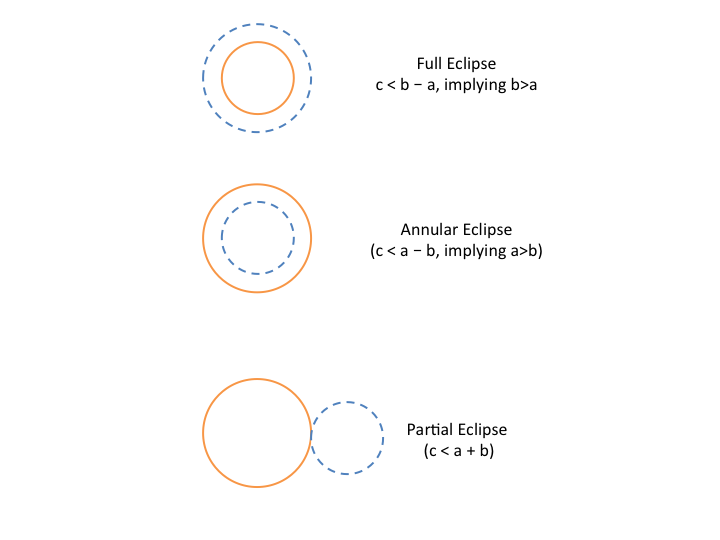
\includegraphics[width=0.9\textwidth]{Figures/diskModel.png}
	\caption{Occultation Disk Model}\label{fig:disk}
\end{figure}
\subsubsection{Total Eclipse ($c < b-a$)}

This type assumes that the apparent radius of the planet is larger than that of the sun ($b>a$). A total eclipse produces a total shadow, so the shadow fraction is 0.0.
\subsubsection{Annular Eclipse ($c < a-b$)}

This type assumes the apparent radius of the sun is larger than that of the planet ($a>b$). Use the equation for a circular area, $A = \pi r^2$, to find the area of the sun and planet faces, replacing $r$ with the corresponding apparent radius. The shadow fraction is then just the ratio of the planet's area to the sun's area.
\begin{equation} \label{eq:18}
Shadow Fraction = \frac{A_P}{A_H}
\end{equation}
\subsubsection{Partial Eclipse ($c < a+ b$)}

For a partial eclipse, the occulted area is given by Eq. \ref{eq:19}.
\begin{equation} \label{eq:19}
A = a^2 \arccos(\frac{x}{a}) + b^2 \arccos(\frac{c-x}{b}) - cy
\end{equation}
Parameters a, b, and c are those calculated previously in Eq. \ref{eq:15}, \ref{eq:16}, and \ref{eq:17}. The values x and y are given by the following equations.
\begin{equation}
x = \frac{c^2 + a^2 - b^2}{2c}
\end{equation}
\begin{equation}
y = \sqrt{a^2 - x^2}
\end{equation}

Like with the annular partial eclipse, the shadow factor for this type is the ratio between the occulted area and the sun's apparent area. This is given by the equation below.
\begin{equation}
Shadow Fraction = 1 - \frac{A}{\pi a^2}
\end{equation}